\documentclass[tikz, border=4pt]{standalone}
\usepackage{amsmath}
\usetikzlibrary{arrows.meta}

% Computational domain and boundary conditions of laminar/powerLaw2d.
% Render the PDF and the SVG used by the user guide next to this file with
%   pdflatex powerLaw2dDomain.tex && pdf2svg powerLaw2dDomain.pdf powerLaw2dDomain.svg

\begin{document}
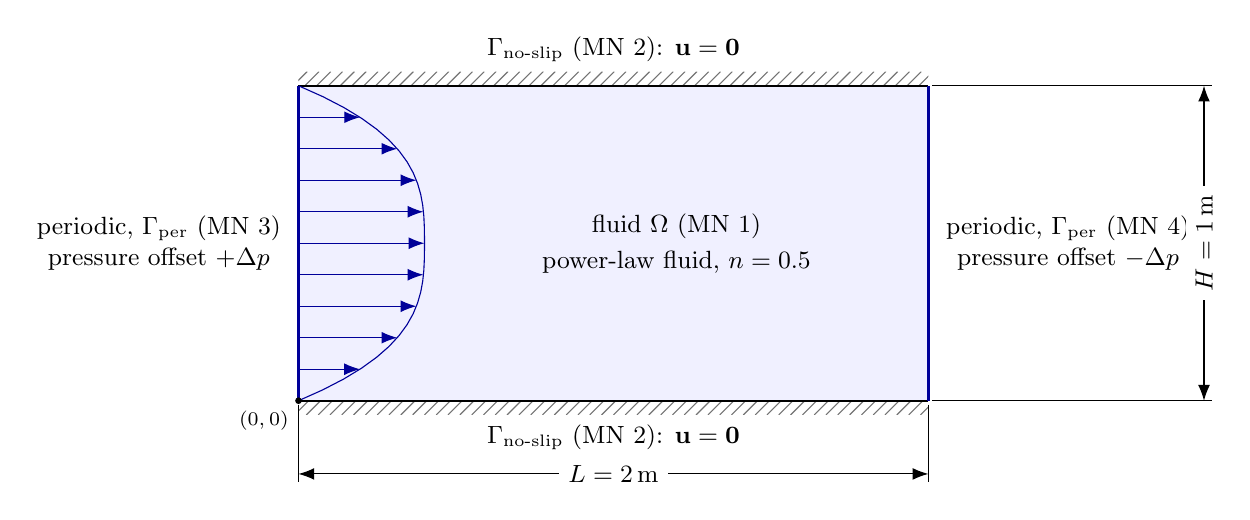
\begin{tikzpicture}[
    >={Latex[length=2mm]},
    dim/.style={<->, thin},
    label/.style={font=\small, align=center},
  ]
  \def\s{4}                       % scale: 1 m = 4 cm
  \pgfmathsetmacro\L{2*\s}        % channel length
  \pgfmathsetmacro\H{1*\s}        % channel height
  \def\w{0.18}                    % thickness of the hatched walls

  % fluid domain
  \fill[blue!6] (0,0) rectangle (\L,\H);

  % walls at the bottom and the top, hatched
  \begin{scope}
    \clip (0,-\w) rectangle (\L,0) (0,\H) rectangle (\L,\H+\w);
    \foreach \x in {-5,-4.85,...,8.2}
      \draw[black!55, thin] (\x,-\w) -- ++(\H+2*\w,\H+2*\w);
  \end{scope}
  \draw[thick] (0,0) -- (\L,0) (0,\H) -- (\L,\H);

  % inflow: parabolic velocity profile
  \draw[very thick, blue!60!black] (0,0) -- (0,\H);
  \foreach \y in {0.1,0.2,...,0.91} {
    \pgfmathsetmacro\u{1.6*(1-abs(2*\y-1)^3)}
    \draw[->, blue!60!black] (0,\y*\H) -- ++(\u,0);
  }
  \draw[blue!60!black, thin, domain=0:1, samples=30]
    plot ({1.6*(1-abs(2*\x-1)^3)}, {\x*\H});

  % outflow
  \draw[very thick, blue!60!black] (\L,0) -- (\L,\H);

  % boundary conditions
  \node[label, left] at (-0.1,0.5*\H)
    {periodic, $\Gamma_\text{per}$ (MN 3)\\ pressure offset $+\Delta p$};
  \node[label, right] at (\L+0.1,0.5*\H)
    {periodic, $\Gamma_\text{per}$ (MN 4)\\ pressure offset $-\Delta p$};
  \node[label, above] at (0.5*\L,\H+\w)
    {$\Gamma_{\mathrm{no\text{-}slip}}$ (MN 2): $\mathbf{u} = \mathbf{0}$};
  \node[label, below] at (0.5*\L,-\w)
    {$\Gamma_{\mathrm{no\text{-}slip}}$ (MN 2): $\mathbf{u} = \mathbf{0}$};

  % fluid
  \node[label] at (0.6*\L,0.5*\H)
    {fluid $\Omega$ (MN 1)\\[2pt] power-law fluid, $n = 0.5$};

  % dimensions
  \draw[dim] (0,-\w-0.75) -- node[fill=white, font=\small] {$L = 2\,\mathrm{m}$} (\L,-\w-0.75);
  \draw[thin] (0,-0.05) -- (0,-\w-0.85) (\L,-0.05) -- (\L,-\w-0.85);
  \draw[dim] (\L+3.5,0) -- node[fill=white, font=\small, rotate=90] {$H = 1\,\mathrm{m}$} (\L+3.5,\H);
  \draw[thin] (\L+0.05,0) -- (\L+3.6,0) (\L+0.05,\H) -- (\L+3.6,\H);

  % origin of the coordinate system
  \fill (0,0) circle (1.2pt) node[below left, font=\scriptsize] {$(0,0)$};
\end{tikzpicture}
\end{document}
